\documentclass[10pt]{mypackage}

\usepackage{mlmodern}
%\usepackage{newpxtext,eulerpx,eucal}
%\renewcommand*{\mathbb}[1]{\varmathbb{#1}}

\usepackage{homework}
%\usepackage{notes}

%\usepackage[ backend=bibtex, style = alphabetic, sorting=ynt ]{biblatex}
%\addbibresource{  }

\usepackage{parskip}

\fancyhf{}
\fancyhead[R]{Avinash Iyer}
\fancyhead[L]{Algebraic Topology: Homework 6}
\fancyfoot[C]{\thepage}

\setcounter{secnumdepth}{0}

\begin{document}
\RaggedRight
\section{Revised Problems from Homework 3}%
\begin{problem}[Problem 1]
  Prove that our cell complex structure for $T^2$ coincides with a product cell complex structure on $S^{1}\times S^{1}$.
\end{problem}
\begin{solution}
  Consider the cell complex structure on $S^1$ given by one $1$-cell, $e^1$, and one $0$-cell, $e^0$, where the endpoints of $e^1$ are identified via the constant map to $e^0$; the corresponding characteristic map is $\Phi\colon [0,1]\rightarrow S^1$, identifying $0\sim 1$.

  Considering two copies of $S^1$ in this fashion, the product CW complex structure is then one consisting of
  \begin{itemize}
    \item one $0$-cell, $e^0_1\times e^0_2$
    \item two $1$-cells, $e^1_1\times e^0_2$ and $e^0_1\times e^1_2$;
    \item one $2$-cell, $e^1_1\times e^1_2$.
  \end{itemize}
  There are then characteristic maps
  \begin{align*}
    \Phi_{1}\colon e^1_1\times e^0_2\rightarrow S^1\times S^1\\
    \Phi_2\colon e^0_1\times e^1_2 \rightarrow S^1\times S^1,
  \end{align*}
  with
  \begin{align*}
    \Phi_1|_{\partial \left( e^1_1\times e^0_2 \right)}\left( e^1_1\times e^0_2 \right) &= e^0_1\times e^0_2\\
    \Phi_2|_{\partial \left( e^0_1\times e^1_2 \right)}\left( e^0_1\times e^1_2 \right) &= e^0_1\times e^0_2.
  \end{align*}
  In particular, this means we may view the $1$-skeleton as a wedge of two circles; since this is difficult to draw in TikZ, we instead simply label all the vertices and edges of the figure below assuming the necessary identifications.
  \begin{center}
    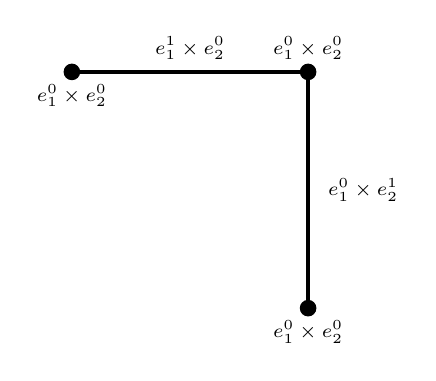
\begin{tikzpicture}
    % Define vertices
    \coordinate (v1) at (0,3);
    \coordinate (v2) at (3,3);
    \coordinate (v3) at (3,0);

    % Draw edges
    \draw[very thick] (v1) -- (v2);
    \draw[very thick] (v2) -- (v3);

    % Draw vertices as filled dots
    \fill (v1) circle (3pt);
    \fill (v2) circle (3pt);
    \fill (v3) circle (3pt);

    % Labels for vertices
    \node at (0,2.7) {\scriptsize $e^0_1\times e^0_2$};
    \node at (3,3.3) {\scriptsize $e^0_1\times e^0_2$};
    \node at (3,-0.3) {\scriptsize $e^0_1\times e^0_2$};

    % Labels for edges
    \node at (1.5,3.3) {\scriptsize $e^1_1\times e^0_2$};
    \node at (3.7,1.5) {\scriptsize $e_1^0\times e^1_2$};
    \end{tikzpicture}
  \end{center}
  The $2$-skeleton is given by $e^{1}_1\times e^1_2$, with a characteristic map $\Psi$ given by the product of the characteristic maps of each of $e^1_1$ and $e^1_2$ (see Hatcher Theorem A.6). Observe that the attaching map is then given by the restriction of $\Psi$ to the boundary, which is 
  \begin{align*}
    \partial \left( e_1^1\times e_2^1 \right) &= \left( e_1^1\times e_2^0 \right)\sqcup \left( e_1^0 \times e_2^1 \right).
  \end{align*}
  Since the $1$-skeleton is precisely $\left( e_1^0\times e_2^1 \right)\sqcup \left( e_1^1\times e_2^0 \right)$, it follows that the attaching map for the $2$-skeleton identifies the boundary of $e_1^1\times e_2^1$ with the $1$-skeleton, giving the following figure:
  \begin{center}
    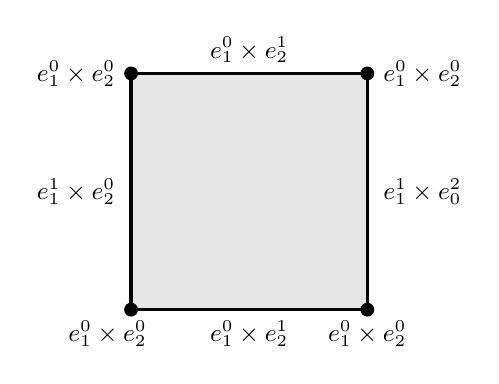
\begin{tikzpicture}
  % Define vertices
  \coordinate (v1) at (0,0);
  \coordinate (v2) at (3,0);
  \coordinate (v3) at (3,3);
  \coordinate (v4) at (0,3);

  % Draw filled square with light gray shading
  \fill[gray!20] (v1) -- (v2) -- (v3) -- (v4) -- cycle;
  % Draw edges
  \draw[very thick] (v1) -- (v2) -- (v3) -- (v4) -- cycle;

  % Draw vertices as filled dots
  \fill (v1) circle (2.5pt);
  \fill (v2) circle (2.5pt);
  \fill (v3) circle (2.5pt);
  \fill (v4) circle (2.5pt);

  % Labels for edges
  \node at (1.5,3.3) {\small $e_1^0\times e_2^1$};
  \node at (3.7,1.5) {\small $e_1^1\times e_0^2$};
  \node at (-0.7,3) {\small $e_1^0\times e_2^0$};
  \node at (3.7,3) {\small $e_1^0\times e_2^0$};
  \node at (3,-0.3) {\small $e_1^0\times e_2^0$};
  \node at (-0.3,-0.3) {\small $e_1^0\times e_2^0$};
  \node at (1.5,-0.3) { \small $e_1^0\times e_2^1$ };
  \node at (-0.7,1.5) { \small $e_1^1\times e_2^0$ };
\end{tikzpicture}
  \end{center}
  which is the cell complex structure of the torus.
\end{solution}
\begin{problem}[Problem 2]
  Prove that if $X$ is a cell complex, then so is the suspension $SX$.
\end{problem}
\begin{solution}
  We observe that the product $X\times [0,1]$ is a cell complex, as it s a Cartesian product of a cell complex with one $1$-cell (the interval itself) and two $0$-cells (the endpoints of the interval). Since the characteristic maps on $X\times [0,1]$ are the products of the characteristic maps on $X$ and $[0,1]$ (see Hatcher Theorem A.6), we see that the attaching maps for $X\times \set{0}$ and $X\times \set{1}$ are the products of the attaching maps for $X$ and the constant maps representing $\set{0}$ and $\set{1}$.

  In particular, this means that $X\times \set{0}$ and $X\times \set{1}$ are subcomplexes of $X\times [0,1]$ (as they contain all their attaching maps). Since the quotient of a cell complex by a subcomplex is a cell complex, it follows that $SX = X\times [0,1]/X\times\set{0}/X\times \set{1}$ is a cell complex.
\end{solution}
\begin{problem}[Problem 3 (b)]
  Prove that $S^{\infty}$ is contractible.
\end{problem}
\begin{solution}
  We view $S^{\infty}$ as the subspace of $\R^{\infty}$, which is the space of finitely supported sequences. Specifically, the space $S^{\infty}$ is the set of the finitely supported sequences $\left( x_n \right)$ such that, if $k$ is the index of the largest nonzero element, then $\left( x_0,\dots,x_k \right)$ is an element of $S^{k}$ --- i.e.,
  \begin{align*}
    \sum_{i=0}^{k}x_i^2 &= 1.
  \end{align*}
  In general, we define the norm of the sequence $\norm{\left( x_n \right)}$ to be the finite sum
  \begin{align*}
    \norm{\left( x_n \right)} &= \sum_{i=0}^{\infty}x_i^2.
  \end{align*}
  Consider now the map $H\colon S^{\infty}\times [0,1]\rightarrow S^{\infty}$
  \begin{align*}
    H\left( \left( x_n \right),t \right) &= \begin{cases}
      \left( 1-2t \right)\left( x_n \right) + 2t \left( x_{n+1} \right) & 0\leq t \leq 1/2\\
      \left( 2-2t \right)\left( x_{n+1} \right) + \left( 2t-1 \right)\left( 1,0,\dots \right) & 1/2\leq t \leq 1.
    \end{cases}
  \end{align*}
  where we insert $0$ into index $0$ in the first half of the homotopy. Then, $H$ is continuous along each of $S^{\infty}\times [0,1/2]$ and $S^{\infty}\times [1/2,1]$ as it is continuous in each variable, and since the piecewise definitions are equal at $t = 1/2$, it follows that $H$ is continuous along $[0,1]$. Then, we see that $H\left(\cdot,t\right)/\norm{H\left(\cdot,t\right)}$ is contained within $S^{\infty}$, and is a homotopy between the identity and a constant map, so the identity is null-homotopic, meaning $S^{\infty}$ is contractible.
\end{solution}
\section{Current Problems}%
\begin{problem}[Problem 1]
  Show that concatenation of paths satisfies the following cancellation property: if $f_0\cdot g_0 \simeq f_1\cdot g_1$, and $g_0\simeq g_1$, then $f_0\simeq f_1$.
\end{problem}
\begin{solution}
  Let $ \overline{g_1} $ denote the reverse path for $g_1$. Then, since $ \overline{g_0}\simeq \overline{g_1} $ as $g_0 \simeq g_1$, we have
  \begin{align*}
    c &\simeq g_0\cdot \overline{g_0}\\
      &\simeq g_0\cdot \overline{g_1}.
  \end{align*}
  In particular, since concatenation is associative, this gives
  \begin{align*}
    f_0 &\simeq f_0\cdot \left( g_0 \cdot \overline{g_0} \right)\\
        &\simeq \left( f_0\cdot g_0 \right)\cdot \overline{g_0}\\
        &\simeq \left( f_1\cdot g_1 \right)\cdot \overline{g_0}\\
        &\simeq f_1\cdot \left( g_1\cdot \overline{g_0} \right)\\
        &= f_1.
  \end{align*}
\end{solution}
\begin{problem}
  Prove that, for a path-connected space $X$, the fundamental group $\pi_1(X)$ is abelian if and only if all the change-of-basepoint isomorphisms $\beta_h$ depend only on the endpoints of the path $h$, not on the precise path.
\end{problem}
\begin{solution}
  Let $X$ be path-connected. Suppose $\pi_1(X)$ is abelian, and let $x_0,x_1$ be distinct points in $X$ with distinct paths $h_1$ and $h_2$ connecting $x_0$ and $x_1$. We will show that $\beta_{h_1}\beta_{ \overline{h_2} }$ is identity on $\pi_1\left( X,x_0 \right)$. Letting $f$ be any loop based at $x_0$, we have
  \begin{align*}
    \beta_{h_1} \beta_{ \overline{h_2} } \left[ f \right] &= \beta_{h_1} \left[ \overline{h_2}\cdot f \cdot h_2 \right]\\
                                                          &= \left[ h_1\cdot \overline{h_2}\cdot f \cdot h_2\cdot \overline{h_1} \right]\\
                                                          &= \left[ h_1\cdot \overline{h_2} \right] \left[ f \right] \left[ h_2\cdot \overline{h_1} \right]\\
                                                          &= \left[ f \right] \left[ h_2\cdot \overline{h_1} \right]\left[ h_1 \cdot \overline{h_2} \right]\\
                                                          &= \left[ f \right].
  \end{align*}
  Thus, $\beta_{h_1} = \beta_{h_2}$.

  Suppose $\beta_{h_1} = \beta_{h_2}$ for any paths $h_1$ and $h_2$ between $x_0$ and $x_1$. We see then that for two loops $f,g$ based at $x_0$
  \begin{align*}
    \left[ f\right]\left[ g \right] &= \left[ f\cdot g \right]\\
                            &= \beta_{h_1} \beta_{ \overline{h_2} } \left[ f\cdot g \right]\\
                            &= \beta_{h_1} \left( \beta_{ \overline{h_2} }\left[ f \right] \beta_{ \overline{h_2} }\left[ g \right]\right)\\
                            &= \beta_{ \overline{h_1} } \left( \left( \beta_{ \overline{h_2} }\left[ f \right] \beta_{ \overline{h_2} }\left[ g \right] \right)^{-1} \right)\\
                            &= \beta_{ \overline{h_1} } \left( \beta_{h_2}\left[ g \right]\beta_{h_2}\left[ f \right] \right)\\
                            &= \beta_{ \overline{h_1} } \beta_{ h_2 } \left[ g\cdot f \right]\\
                            &= \left[ g\cdot f \right]\\
                            &= \left[ g \right]\left[ f \right].
  \end{align*}
\end{solution}
\end{document}
